\documentclass[11pt,a4paper]{article}
\usepackage[utf8]{inputenc}
\usepackage[top=0.70in, bottom=0.70in, left=0.8in,right=0.80in]{geometry} 
\usepackage[pdftex]{graphicx} 
\usepackage[final]{pdfpages} 
\usepackage{float} 
\usepackage{hyperref}
\hypersetup{pdfborder = {0 0 0}}
%\usepackage{pslatex} 
\usepackage{array} 
\usepackage{tabularx}
\usepackage{booktabs}
\usepackage{ragged2e}
\usepackage{setspace}
%\usepackage{float}
\usepackage{enumerate}
\usepackage{enumitem}
\usepackage{longtable}
\usepackage{placeins}
\usepackage{microtype}
\usepackage[english]{babel}
\usepackage{amsmath}
\usepackage{pgfpages}
\usepackage[font=small,labelfont=bf]{caption}
\def\figurename{\textbf{Figure }}
%Includes "References" in the table of contents
\usepackage[nottoc]{tocbibind}
%for creating Abbreviation
\usepackage{acronym}

\usepackage{listings}
\usepackage{color}

\definecolor{dkgreen}{rgb}{0,0.6,0}
\definecolor{gray}{rgb}{0.5,0.5,0.5}
\definecolor{mauve}{rgb}{0.58,0,0.82}
 

%For the header and footer
\usepackage{fancyhdr}
%\fancypagestyle{fancy}{%
%\fancyfoot[L]{\emph{Department of Computer Engineering, SHORT NAME OF COLLEGE, Pune}} % except the center
%\fancyfoot[R]{\thepage}
%\renewcommand{\headrulewidth}{0.4pt}
%\renewcommand{\footrulewidth}{0.4pt}
%}

\pagestyle{fancy}

\rhead{\large{Automated Cooking Assistant With AI}}
\fancyhead[L]{}
\fancyfoot[R]{\emph{Department of MCA}}
%\cfoot{}
\fancyfoot[C]{\thepage}
\renewcommand{\headrulewidth}{0.5pt}
\renewcommand{\footrulewidth}{0.5pt}
%Page Border
% 
\addto\captionsenglish{\renewcommand*\contentsname{\centering{Contents}}}
\addto\captionsenglish{
\renewcommand{\listfigurename}{\textit{List of Figures}}
}

\addto\captionsenglish{
\renewcommand{\listtablename}{\textit{List of Tables}}
}



%GLOBAL SETTINGS OVER, DOCUMENT BEGINS
\begin{document}
\justifying
\onehalfspacing
\setlength{\parindent}{0pt}
\setlength{\parskip}{6pt}
\setlist[itemize]{leftmargin=*, itemsep=3pt, topsep=3pt}
\setlist[enumerate]{leftmargin=*, itemsep=3pt, topsep=3pt}
\renewcommand{\arraystretch}{1.18}
%\renewcommand\bibname{References}
%\lhead{ }

%FROM HERE YOUR PAGES START GETTING ADDED
%\pgfpagesuselayout{boxed}
%\setlength{\parindent}{1cm}
% includes the cover page
%\pgfpagesuselayout{boxed}
%\input{project/cover.tex}
\pagenumbering{roman} %numbering before main content starts

\newpage
\begin{center}
\thispagestyle{empty}
\Large{\textbf{A  PROJECT CASED LEARNING REPORT \\ON}}\\[0.2cm]
\Large{\textsc {\textbf{``AUTOMATED COOKING ASSISTANT WITH AI''}}}\\
\vspace{0.1cm}

\includegraphics[scale=.5]{uop-logo}\\
\Large{\textbf{\\Submitted to}}
\LARGE{\textbf{\\ SAVITRIBAI PHULE PUNE UNIVERSITY\\}}
\large{\textbf{\\In Partial Fulfilment of the Requirement for the Award of\\}}
\Large{\textbf{\\ MASTER OF COMPUTER APPLICATIONS (Under Engineering)}}
\vspace{0.3cm}
\Large{\textbf{\\BY}}\\[0.1cm]
\begin{table}[h]
\centering
\Large{\textbf{
%\begin{tabular}{>{\bfseries}lc>{\bfseries}r}
 \textbf{Vaibhav  Shinde}\\
        \textbf{Shivam Gautam}\\
        \textbf{Rushab Yadav}\\
        \textbf{Suraj Yadav}\\
%\end{tabular}
}}
\end{table}
\large{\textbf{UNDER THE GUIDANCE OF}}\\
\Large{\textbf{ Prof. Dipali Bhusari }}\\[0.1cm]

\includegraphics[scale=0.3]{tae.png}\\[.5cm]
\large{\textbf{DEPARTMENT OF MASTER OF COMPUTER APPLICATIONS}}\\
\Large{\textbf{TRINITY ACADEMY OF ENGINEERING}}\\[.5cm]
\large{\textbf{Kondhwa Annex, Pune - 411048}}
\large{\textbf{\\2024-2025}}\\

%\Large{\textbf{NAME OF COLLEGE}}\\
%\large{\textbf{LOCATION IN PUNE, PUNE - PINCODE}}
%\large{\textbf{\\2021-2022}}\\[0.5cm]
%\Large{\textbf{AFFILIATED TO}}\\[0.5cm]
%
\includegraphics[scale=.5]{project/images/uop-logo}\\
%\LARGE{\textbf{UNIVERSITY OF PUNE}}
\newpage

\end{center}
\newpage

% includes the certificate page
\begin{center}
\thispagestyle{empty}

\LARGE{\textbf{TRINITY ACADEMY OF ENGINEERING}} \\ 
\large{\textbf{Department of Master of Computer Applications}}\\


\includegraphics[scale=0.3]{tae.png}\\[1cm]

{\Huge \textbf{CERTIFICATE}}\\[0.5cm]
\end{center}
\linespread{1.13}
\large{\centering{This is certify that the Major Project entitled}\\[0.2cm]
\textbf{\Large{\centering{``AUTOMATED COOKING ASSISTANT WITH AI``}}}\\
\centering{has successfully submitted by}\\
\begin{table}[h]
\centering
\large{\textbf{Vaibhav  Shinde}\\
        \textbf{Shivam Gautam}\\
        \textbf{Rushab Yadav}\\
        \textbf{Suraj Yadav}\\
        }
\end{table}
 under the supervision of \textbf{Prof.Dipali Bhusari} and it is approved for the partial fulfillment of the
requirement of Savitribai Phule Pune University, for the award of the degree of Master of
Computer Applications (Under Engineering).}\\[0.5cm]
\large{\textbf{Date:\hspace*{0.4cm}/\hspace*{0.4cm}/}}\\[.2cm]
%\vspace*{0.4cm}
\large{\textbf{Place: Pune}}\\
\begin{spacing}{0}
%\vspace{0.8cm}
\vspace*{1.2cm}
\hspace*{0.3in}\large{\textbf{Dipali Bhusari}}\hspace {1.1in}\large{\textbf{Dr. A. A. Bhusari}}\hspace*{1 in}\large{\textbf{Dr. R. J. Patil}}\\[.1cm]
%\vspace*{.3cm}
\hspace*{0.4in}\textbf{Project Guide}\hspace*{1.8in}\textbf{HOD} \hspace*{1.5in}\textbf{Principal}\\
\hspace*{0.1 in}\textbf{Department of MCA}\hspace*{.8in}\textbf{Department of MCA} \hspace*{.9in}\textbf{TAE, Pune}\\[1 cm]
This project report has been examined by us as per the Savirtibai Phule Pune University, Pune,
requirements at Trinity Academy of Engineering, Pune.
\\[2 cm]
\hspace*{0.5in}\textbf{Internal Examiner} \hspace*{2.6in}
%\hspace*{0.3in}\large{\textbf{(Dr. N J Uke)}}\\
%\hspace*{0.4in}\textbf{Principal}
%\hspace*{2.5in}\textbf{External Examiner}\\[1.0cm]
\end{spacing}

 
\addcontentsline{toc}{section}{\textit{Certificate}}
\newpage

% includes the acknowledgements page
\begin{center}
\thispagestyle{plain}
\LARGE{\textbf{Acknowledgement}}\\[1cm]
\end{center}
\linespread{1.13}
\large{\paragraph{}
I would like to acknowledge all the teacher and friends who ever helped and assisted me throughout my project work.\newline \newline
First of all I would like to thank my respected guide \textbf {Prof. Dipali Bhusari}, introducing me throughout features needed. The time-to-time guidance, encouragement and valuable suggestion received from him are unforgettable in my life. This work would not have been possible without the enthusiastic response, insight and new idea from him.\newline \newline
Furthermore, I would like to thank respected \textbf{Dr. R. J. Patil}, Principal and  \textbf{Dr. A. A. Bhusari}, Head of Department of Master of Computer Applications for the guidance provided by them during my project work. I am also grateful to all the faculty members of Trinity Academy of Engineering, Pune for their support and cooperation. I would like to thank my lovely parent for time-to-time support and encouragement and valuable suggestion, and I would specify like to thank all my friends for their valuable suggestion and support. The acknowledgement world be incomplete without mention of the blessing of the almighty, which helped me in keeping high moral during difficult period.
}
\large{\paragraph{}
}
\begin{flushright}
    \begin{minipage}{0.45\textwidth}
        \textbf{Candidates:}\\[0.5cm]
        \textbf{Vaibhav  Shinde}\\
        \textbf{Shivam Gautam}\\
        \textbf{Rushab Yadav}\\
        \textbf{Suraj Yadav}\\[0.8cm]
        \textbf{Seat Numbers: \hrulefill}\\
        \textbf{Department of MCA}
    \end{minipage}
\end{flushright}
%\newpage

\addcontentsline{toc}{section}{\textit{Acknowledgements}}
\newpage
\thispagestyle{empty} % Declaration pages usually don't have page numbers

\begin{center}
    \vspace*{1.8cm}
    {\LARGE \textbf{Declaration by the Candidates}}\\[1.5cm]
\end{center}

\linespread{1.5} % Increased for better readability in formal declarations
\large
We hereby declare that this project report titled \textbf{"AUTOMATED COOKING ASSISTANT WITH AI"} submitted towards partial fulfillment of requirements for the degree of \textbf{Master of Computer Applications (MCA)} is an authentic record of our work carried out under the guidance of \textbf{Prof. Dipali Bhusari}.

\vspace{0.5cm}
We further declare that the material obtained from other resources is duly acknowledged in this report.

\vspace{1.5cm}

\noindent \textbf{Date: \hspace{0.5cm} / \hspace{0.5cm} /} \\
\textbf{Place: Pune}

\vspace{-1cm} % Adjusts vertical alignment for the names

\begin{flushright}
    \begin{minipage}{0.45\textwidth}
        \textbf{Candidates:}\\[0.5cm]
        \textbf{Vaibhav  Shinde}\\
        \textbf{Shivam Gautam}\\
        \textbf{Rushab Yadav}\\
        \textbf{Suraj Yadav}\\[0.8cm]
        \textbf{Seat Numbers: \hrulefill}\\
        \textbf{Department of MCA}
    \end{minipage}
\end{flushright}
\addcontentsline{toc}{section}{\textit{Declaration}}
\newpage

\begin{center}
\thispagestyle{plain}
\vspace{2cm}
\LARGE{\textbf{Abstract}}\\[1.0cm]
\end{center}
The AI Recipe Generator is a web-based application designed to help users create
recipes from available ingredients, dietary preferences, cuisine choices, cooking
time, and serving requirements. The system reduces the everyday difficulty of deciding
what to cook by combining a clean user interface with AI-assisted recipe generation.\\
The application provides user authentication, profile management, pantry tracking,
recipe generation, saved recipes, shopping list support, meal planning, and preference
management. The frontend is developed using React, Vite, Tailwind CSS, React Router,
Axios, and Lucide icons. The backend uses Node.js, Express.js, JWT authentication,
bcrypt password hashing, PostgreSQL, Sequelize, and the Google GenAI package for AI
integration.\\
The project focuses on usability, personalization, data security, and practical meal
planning. It supports a structured database design for users, preferences, pantry
items, recipes, nutrition, meal plans, and shopping lists. \newline\\
 

\textit{{\textbf{Keywords: }}- AI, recipe generation, meal planning, pantry management, React, Express,
PostgreSQL, JWT.} % adds the Research Methodology page
\addcontentsline{toc}{section}{\textit{Abstract}}
\newpage
%\stepcounter{page}


%TABLE OF CONTENTS AND LIST OF FIGURES ARE AUTOMATICALLY ADDED BY FOLLOWING COMMANDS
%ADD FIGURE OF TABLES IF YOU NEED TO, CHECK DOCUMENTATION

%To reset the Header & Footer for TOC and LOF
\pagestyle{empty}
%\addtocontents{toc}{\protect\thispagestyle{empty}}

\tableofcontents % adds Index Page 
\newpage
\listoffigures % adds List of Figures
\newpage
\listoftables  % adds List of Tables
%\addtocontents{lof}{}
\newpage
\thispagestyle{plain}
\section*{List of Abbreviation}
\begin{acronym}[HSHRP] % Give the longest label here so that the list is nicely aligned
\acro{AI}{Artificial Intelligence}
\acro{API}{Application Programming Interface}
\acro{DBMS}{Database Management System}
\acro{DFD}{Data Flow Diagram}
\acro{ERD}{Entity Relationship Diagram}
\acro{JWT}{JSON Web Token}
\acro{SRS}{Software Requirements Specification}
\acro{UI}{User Interface}
\end{acronym}
\addcontentsline{toc}{section}{\textit{List of Abbreviation}}
\newpage
\cleardoublepage

%And reset back the settings we choose for Header and Footer
\pagestyle{fancy}

\newpage
\pagenumbering{arabic} %reset numbering to normal for the main content

\section{About Project}

\subsection{Title}
\textbf{Automated Cooking Assistant with AI}

\subsection{Domain}
Artificial Intelligence, Food Technology, Web Application Development, Personal Productivity, and Meal Planning.

\subsection{Aim}
\begin{itemize}
\item To develop an AI-based recipe generation system that suggests recipes from available ingredients and user preferences.
\item To provide an integrated cooking assistant with pantry management, saved recipes, meal planning, and shopping list support.
\end{itemize}

\subsection{Objective}
The objective of this project is to build a secure and user-friendly web application that generates personalized recipes, stores user preferences, manages pantry items, saves useful recipes, plans meals, and prepares shopping lists so that users can make better use of available ingredients and reduce daily meal planning effort.

\subsection{Problem Statement}
Many users find it difficult to decide what to cook with ingredients already available at home. The decision becomes harder when dietary restrictions, preferred cuisine, cooking time, and serving size must also be considered.

Existing recipe websites mainly depend on manual search and fixed recipe collections. They often do not combine pantry tracking, AI-based recipe creation, meal planning, saved recipes, and shopping lists in a single workflow.

This project proposes an intelligent web application that generates personalized recipes from available ingredients and user preferences. By integrating pantry management, meal planning, and shopping list support, the system improves convenience, reduces waste, and makes everyday cooking more organized.
 % adds the introduction page
\newpage
\section{Introduction}

\subsection{Overview}
The AI Recipe Generator is a full-stack web application that helps users create recipes from available ingredients and personal food preferences. The frontend is built with React and Vite, while the backend uses Express.js, PostgreSQL, Sequelize, JWT authentication, and AI service integration.

\subsection{Motivation}
Food waste and meal decision fatigue are common daily problems. A user may have ingredients available but may not know how to combine them into a complete dish. This project makes cooking decisions faster, more personal, and better organized.

\subsection{Project Scope \& Limitations}
\textbf{Project Scope}

The application includes user registration, login, profile management, preference management, pantry tracking, recipe generation, saved recipes, meal planning, and shopping list support.

The frontend provides pages for Login, Signup, Dashboard, Recipe Generator, Pantry, My Recipes, Meal Planner, Shopping List, Recipe Details, and Settings. The backend provides REST APIs for authentication, user data, preferences, pantry records, recipes, and planning features.

The database stores structured data such as users, preferences, pantry items, recipes, ingredients, nutrition details, meal plans, and shopping lists.

\textbf{Project Limitations}
\begin{itemize}
\item Recipe quality depends on the AI model, entered ingredients, and selected preferences.
\item Internet access and valid API configuration are required for real-time AI generation.
\item Nutrition and diet suggestions are supportive and should not replace professional medical advice.
\item Production deployment would require additional security review, performance tuning, and monitoring.
\item Advanced features such as barcode scanning, voice commands, image-based ingredient detection, and online grocery ordering are outside the current scope.
\end{itemize}

\subsection{Methodology of Problem Solving}
The project follows a modular development approach. First, the main user problem is identified: users need quick, personalized recipe ideas based on available ingredients. The system requirements are then divided into modules such as authentication, recipe generation, pantry management, saved recipes, meal planner, shopping list, and settings.

The frontend is designed in React to provide a responsive interface, while the backend is implemented in Node.js and Express.js to handle API requests. PostgreSQL stores user accounts, preferences, pantry items, recipes, meal plans, and shopping lists.

After login, the user enters ingredients or selects pantry items. Preferences such as cuisine, diet, serving size, and cooking time are sent to the AI service. The generated recipe is displayed with ingredients, instructions, time, difficulty, and nutrition details. The user can then save the recipe, plan it for a meal, or add missing ingredients to a shopping list. Important workflows are tested iteratively to improve correctness and usability.

\newpage

\section{Literature Survey}

\subsection{Similar Work}
Existing recipe platforms provide searchable collections of dishes, ingredients, and cooking instructions \cite{allrecipes}. Meal planning applications help users organize weekly meals and grocery lists \cite{mealime}. AI services can generate text-based recipe ideas from user prompts and ingredient lists \cite{googleai}. However, these systems usually focus on separate parts of the cooking workflow. The proposed AI Recipe Generator combines recipe generation, user preferences, pantry management, saved recipes, meal planning, and shopping list support in one system.

\subsection{Tabulated Short Survey}
\begin{table}[h]
\centering
\caption{Tabulated Short Survey}
\begin{tabularx}{\textwidth}{|p{3.8cm}|X|X|}
\hline
\textbf{System} & \textbf{Features} & \textbf{Limitations} \\
\hline
Traditional Recipe Websites \cite{allrecipes} & Search recipes by name, cuisine, ingredients, and category. & Less personalized and mostly require manual searching and filtering. \\
\hline
Meal Planner Applications \cite{mealime} & Provide calendar-based meal planning and grocery list preparation. & Recipe creation is limited and usually depends on existing recipe collections. \\
\hline
AI Recipe/Chat Tools \cite{googleai} & Generate recipe text from prompts and ingredient lists. & Do not provide complete pantry management, saved recipes, or structured planning. \\
\hline
Proposed AI Recipe Generator & Provides AI recipe generation, preferences, pantry, saved recipes, meal planning, and shopping list support. & Requires internet access and proper AI API integration. \\
\hline
\end{tabularx}
\end{table}

\subsection{Outcome of Literature Survey}
\begin{enumerate}
\item Existing recipe websites are useful, but users still need manual searching and filtering.
\item Meal planning tools are helpful, but they rarely generate new recipes from available ingredients.
\item AI tools can create recipe ideas, but they usually lack structured storage, pantry tracking, and meal planning.
\item The proposed system addresses this gap by combining recipe generation and meal organization in one application.
\end{enumerate}
 % adds the Literature Survey page

\newpage
%\input{project/req-analysis.tex}
%\section{System Design}
\paragraph{} WRITE HERE.

\newpage
\section{Software Requirements Specification}

\subsection{System Specific Requirements}
\begin{table}[h]
\centering
\caption{System Specific Requirements}
\begin{tabularx}{\textwidth}{|p{4cm}|X|}
\hline
\textbf{Requirement} & \textbf{Description} \\
\hline
User Authentication & Users can register, log in, and access protected pages using JWT authentication. \\
\hline
Recipe Generation & The system generates recipes using ingredients, cuisine, dietary tags, servings, and cooking time. \\
\hline
Pantry Management & Users can add, update, and manage pantry ingredients. \\
\hline
Meal Planning & Users can plan meals and connect selected recipes with daily meal slots. \\
\hline
Shopping List & The system supports grocery list preparation based on recipe and pantry needs. \\
\hline
Database Storage & User profiles, preferences, pantry items, saved recipes, meal plans, and shopping lists are stored in PostgreSQL. \\
\hline
\end{tabularx}
\end{table}

\subsection{Hardware Requirements}
\begin{table}[h]
\centering
\caption{Hardware Requirements}
\begin{tabularx}{\textwidth}{|p{4cm}|X|}
\hline
\textbf{Hardware} & \textbf{Requirement} \\
\hline
Processor & Intel Core i3 or above. \\
\hline
RAM & Minimum 4 GB. \\
\hline
Storage & Minimum 500 MB free space. \\
\hline
Internet & Stable internet connection for API and database operations. \\
\hline
Display & 1366 $\times$ 768 resolution or above. \\
\hline
Input Devices & Keyboard and mouse. \\
\hline
\end{tabularx}
\end{table}

\subsection{Software Requirements}
\begin{table}[h]
\centering
\caption{Software Requirements}
\begin{tabularx}{\textwidth}{|p{4cm}|X|}
\hline
\textbf{Software} & \textbf{Requirement} \\
\hline
Operating System & Windows, Linux, or macOS. \\
\hline
Frontend & React.js, Vite, Tailwind CSS, React Router, Axios. \\
\hline
Backend & Node.js and Express.js. \\
\hline
Database & PostgreSQL with Sequelize ORM. \\
\hline
Authentication & JWT and bcrypt password hashing. \\
\hline
AI Service & Google GenAI/Gemini API. \\
\hline
Development Tools & Visual Studio Code, npm, Git, Postman. \\
\hline
Browser & Google Chrome, Microsoft Edge, Mozilla Firefox, or any modern browser. \\
\hline
\end{tabularx}
\end{table}

\FloatBarrier

\newpage
\section{Project Plan}

\subsection{Project Estimate}
The project is divided into requirement analysis, UI design, backend setup, database design, authentication, AI recipe generation, testing, and documentation.

\subsubsection{Reconciled Estimates}
\begin{table}[h]
\centering
\caption{Reconciled Estimates}
\begin{tabularx}{\textwidth}{|X|p{3cm}|p{3cm}|}
\hline
\textbf{Project Activity} & \textbf{Estimated Time} & \textbf{Final Estimate} \\
\hline
Requirement Analysis & 1 Week & 1 Week \\
\hline
System Design & 1 Week & 1 Week \\
\hline
Frontend Development & 2 Weeks & 2 Weeks \\
\hline
Backend Development & 2 Weeks & 2 Weeks \\
\hline
Database Design & 1 Week & 1 Week \\
\hline
AI API Integration & 1 Week & 1 Week \\
\hline
Testing and Documentation & 2 Weeks & 2 Weeks \\
\hline
\textbf{Total} & \textbf{10 Weeks} & \textbf{10 Weeks} \\
\hline
\end{tabularx}
\end{table}

\subsubsection{Project Resources}
\begin{table}[h]
\centering
\caption{Project Resources}
\begin{tabularx}{\textwidth}{|p{4cm}|X|}
\hline
\textbf{Resource Type} & \textbf{Resources Used} \\
\hline
Human Resources & Student developer, project guide, faculty members. \\
\hline
Hardware Resources & Laptop or desktop computer, keyboard, mouse, internet connection. \\
\hline
Software Resources & Visual Studio Code, Node.js, React.js, Express.js, PostgreSQL, Git, Postman. \\
\hline
Database Resources & PostgreSQL database, Sequelize ORM. \\
\hline
API Resources & Google GenAI/Gemini API for recipe generation. \\
\hline
\end{tabularx}
\end{table}

\FloatBarrier
\subsection{Risk Management}
\begin{table}[h]
\centering
\caption{Risk Management}
\begin{tabularx}{\textwidth}{|p{3.6cm}|p{4cm}|X|}
\hline
\textbf{Risk} & \textbf{Impact} & \textbf{Mitigation Strategy} \\
\hline
API Failure & Recipe generation may stop working. & Handle API errors and show clear messages. \\
\hline
Database Failure & User data may not be saved or retrieved. & Use constraints, backups, and connection error handling. \\
\hline
Security Risk & Unauthorized access to user data. & Use JWT authentication, password hashing, and protected routes. \\
\hline
Poor Performance & Application may load slowly. & Optimize database queries and frontend assets. \\
\hline
Invalid User Input & Incorrect data may affect output. & Validate input on frontend and backend. \\
\hline
Schedule Delay & Project completion may be delayed. & Complete modules phase-wise and review progress regularly. \\
\hline
\end{tabularx}
\end{table}
\FloatBarrier

\newpage
\section{System Design}

This section presents the main design diagrams of the proposed AI Recipe Generator system.

\subsection{System Architecture}
The system architecture shows the interaction between the React frontend, Express backend, PostgreSQL database, authentication layer, and AI service.

\begin{figure}[htbp]
    \centering
    \includegraphics[width=0.9\linewidth,height=0.45\textheight,keepaspectratio]{Gemini_Generated_Image_2dzvgc2dzvgc2dzv.png}
    \caption{System Architecture}
    \label{fig:sys_arch}
\end{figure}

\FloatBarrier
\subsection{Data Flow Diagram}
The data flow diagram shows how user input, pantry data, recipe requests, generated output, and stored records move through the system.

\begin{figure}[htbp]
    \centering
    \includegraphics[width=0.9\linewidth,height=0.45\textheight,keepaspectratio]{Gemini_Generated_Image_6c1usc6c1usc6c1u.png}
    \caption{Data Flow Diagram}
    \label{fig:dfd}
\end{figure}

\FloatBarrier
\subsection{ER Diagram}
The ER diagram represents the major database entities and relationships used in the project.

\begin{figure}[H]
\centering
\fbox{%
\begin{minipage}{0.92\textwidth}
\centering
\small
\begin{tabular}{c c c}
\fbox{\begin{minipage}{0.26\textwidth}\centering\textbf{Users}\\user\_id\\name\\email\\password\end{minipage}}
&
$1:N$
&
\fbox{\begin{minipage}{0.26\textwidth}\centering\textbf{User Preferences}\\preference\_id\\diet\\allergies\\cuisine\end{minipage}}
\\[1.2cm]
\fbox{\begin{minipage}{0.26\textwidth}\centering\textbf{Pantry Items}\\pantry\_id\\ingredient\\quantity\\user\_id\end{minipage}}
&
$N:1$
&
\fbox{\begin{minipage}{0.26\textwidth}\centering\textbf{Recipes}\\recipe\_id\\title\\instructions\\user\_id\end{minipage}}
\\[1.2cm]
\fbox{\begin{minipage}{0.26\textwidth}\centering\textbf{Meal Plans}\\plan\_id\\date\\meal\_type\\recipe\_id\end{minipage}}
&
$N:1$
&
\fbox{\begin{minipage}{0.26\textwidth}\centering\textbf{Shopping List}\\list\_id\\item\\quantity\\user\_id\end{minipage}}
\end{tabular}

\vspace{0.5cm}
Users maintain preferences, pantry items, recipes, meal plans, and shopping list records. Recipes are connected with meal plans, while pantry and shopping data support ingredient management.
\end{minipage}}
\caption{ER Diagram}
\label{fig:er_diagram}
\end{figure}

\FloatBarrier

\newpage
\section{Implementation}

The AI Recipe Generator is implemented as a web-based application using a React.js frontend and a Node.js backend. The system allows users to register, log in, enter ingredients, set food preferences, generate recipes using AI, save recipes, manage pantry items, prepare meal plans, and create shopping lists.

\subsection{Frontend Implementation}

The frontend is developed using React.js with Vite for fast development and build support. Tailwind CSS is used for designing responsive and user-friendly pages. React Router is used for navigation between pages such as Login, Signup, Dashboard, Recipe Generator, Pantry, Meal Planner, My Recipes, Shopping List, and Settings.

Axios is used to communicate with the backend API. The JWT token received after login is stored on the client side and sent with protected API requests.

\subsection{Backend Implementation}

The backend is developed using Node.js and Express.js. It provides REST API endpoints for user registration, login, profile management, preferences, and other application features. Express middleware is used for JSON parsing, CORS handling, and authentication.

JWT authentication is used to protect private routes. Passwords are hashed before storing in the database to improve security.

\subsection{Database Implementation}

PostgreSQL is used as the database for storing user data, preferences, recipes, pantry items, meal plans, and shopping lists. Sequelize ORM is used to define models and perform database operations. Primary keys, foreign keys, and constraints are used to maintain data integrity.

\subsection{AI Integration}

The system integrates Google GenAI/Gemini API for recipe generation. User-provided ingredients, cuisine type, dietary restrictions, cooking time, and serving size are sent to the AI service. The generated recipe is returned and displayed to the user.

\subsection{Authentication Implementation}

User authentication is handled using JWT tokens. After successful login, the server generates a token and sends it to the frontend. This token is included in the Authorization header for protected requests.

\subsection{Module Implementation}

The main modules implemented in the system are:

\begin{itemize}
    \item User Registration and Login
    \item User Profile and Preferences
    \item Recipe Generation
    \item Pantry Management
    \item Saved Recipes
    \item Meal Planning
    \item Shopping List Management
\end{itemize}

%\input{project/implementation.tex} % adds the Project Design
%\input{project/screenshots.tex}
\newpage
\section{Software Testing}

Software testing verifies that the AI Recipe Generator works according to the project requirements. The testing focused on authentication, protected access, recipe generation, pantry management, meal planning, shopping list creation, and profile updates.

\subsection{Testing Objectives}
\begin{itemize}
\item To verify that all implemented modules work according to the requirements.
\item To check user registration, login, and protected page access.
\item To validate recipe generation using user inputs.
\item To check database storage and retrieval of user data.
\item To ensure the application is user-friendly and responsive.
\end{itemize}

\subsection{Test Cases}
\begin{table}[h]
\centering
\caption{Test Cases}
\begin{tabularx}{\textwidth}{|p{1.5cm}|X|X|p{2cm}|}
\hline
\textbf{Test ID} & \textbf{Test Case} & \textbf{Expected Result} & \textbf{Status} \\
\hline
T1 & User registration with valid details. & Account should be created successfully. & Pass \\
\hline
T2 & User login with valid credentials. & User should log in and receive JWT token. & Pass \\
\hline
T3 & Login with invalid password. & Error message should be displayed. & Pass \\
\hline
T4 & Access protected page without token. & Access should be denied. & Pass \\
\hline
T5 & Generate recipe using ingredients. & Recipe should be generated successfully. & Pass \\
\hline
T6 & Save generated recipe. & Recipe should be saved in database. & Pass \\
\hline
T7 & Add pantry item. & Pantry item should be stored successfully. & Pass \\
\hline
T8 & Create meal plan. & Meal plan should be created successfully. & Pass \\
\hline
T9 & Generate shopping list. & Shopping list should be displayed correctly. & Pass \\
\hline
T10 & Update user profile. & Profile details should be updated successfully. & Pass \\
\hline
\end{tabularx}
\end{table}

\FloatBarrier

\newpage
\section{Output Screens}

The following screens show the main user flow of the AI Recipe Generator, from authentication to recipe planning and configuration.

\subsection{User Authentication}
\begin{figure}[htbp]
    \centering
    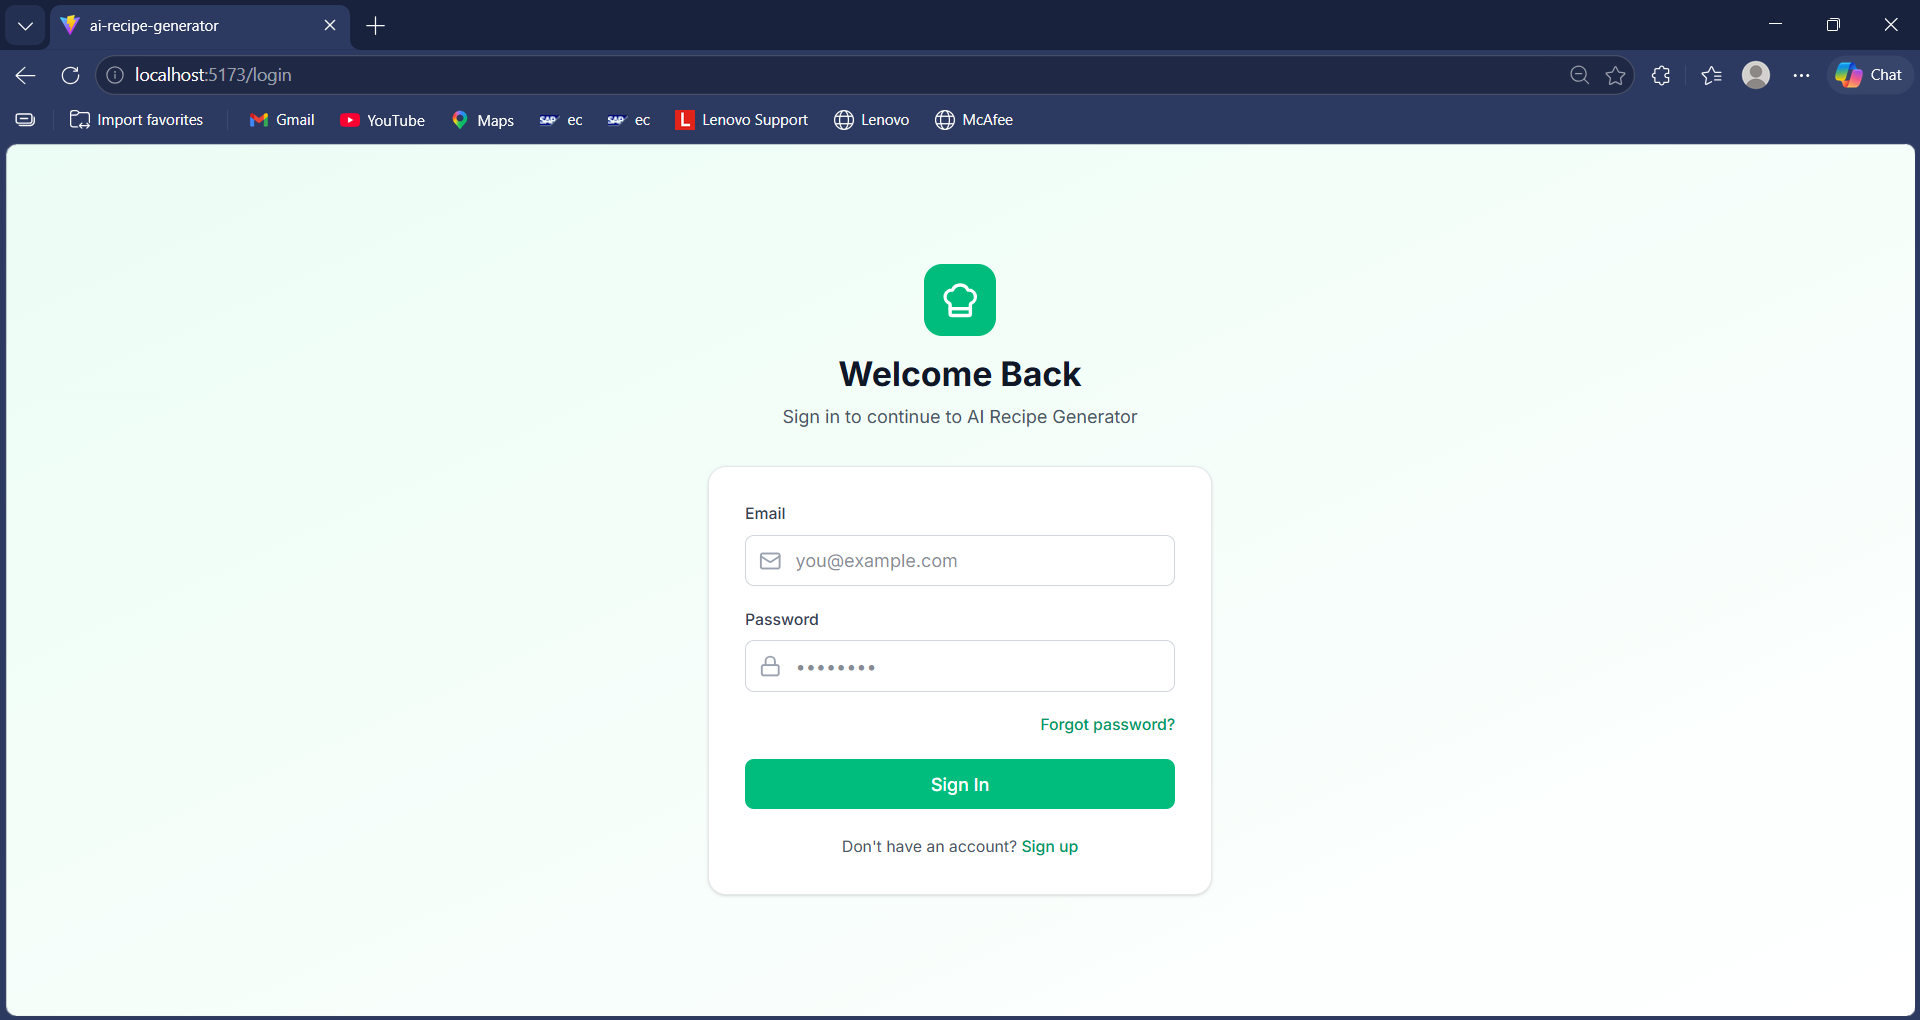
\includegraphics[width=0.78\textwidth,height=0.36\textheight,keepaspectratio]{Screenshot 2026-05-07 223328.png}
    \caption{User Login Interface}
    \label{fig:login_screen}
\end{figure}

\begin{figure}[htbp]
    \centering
    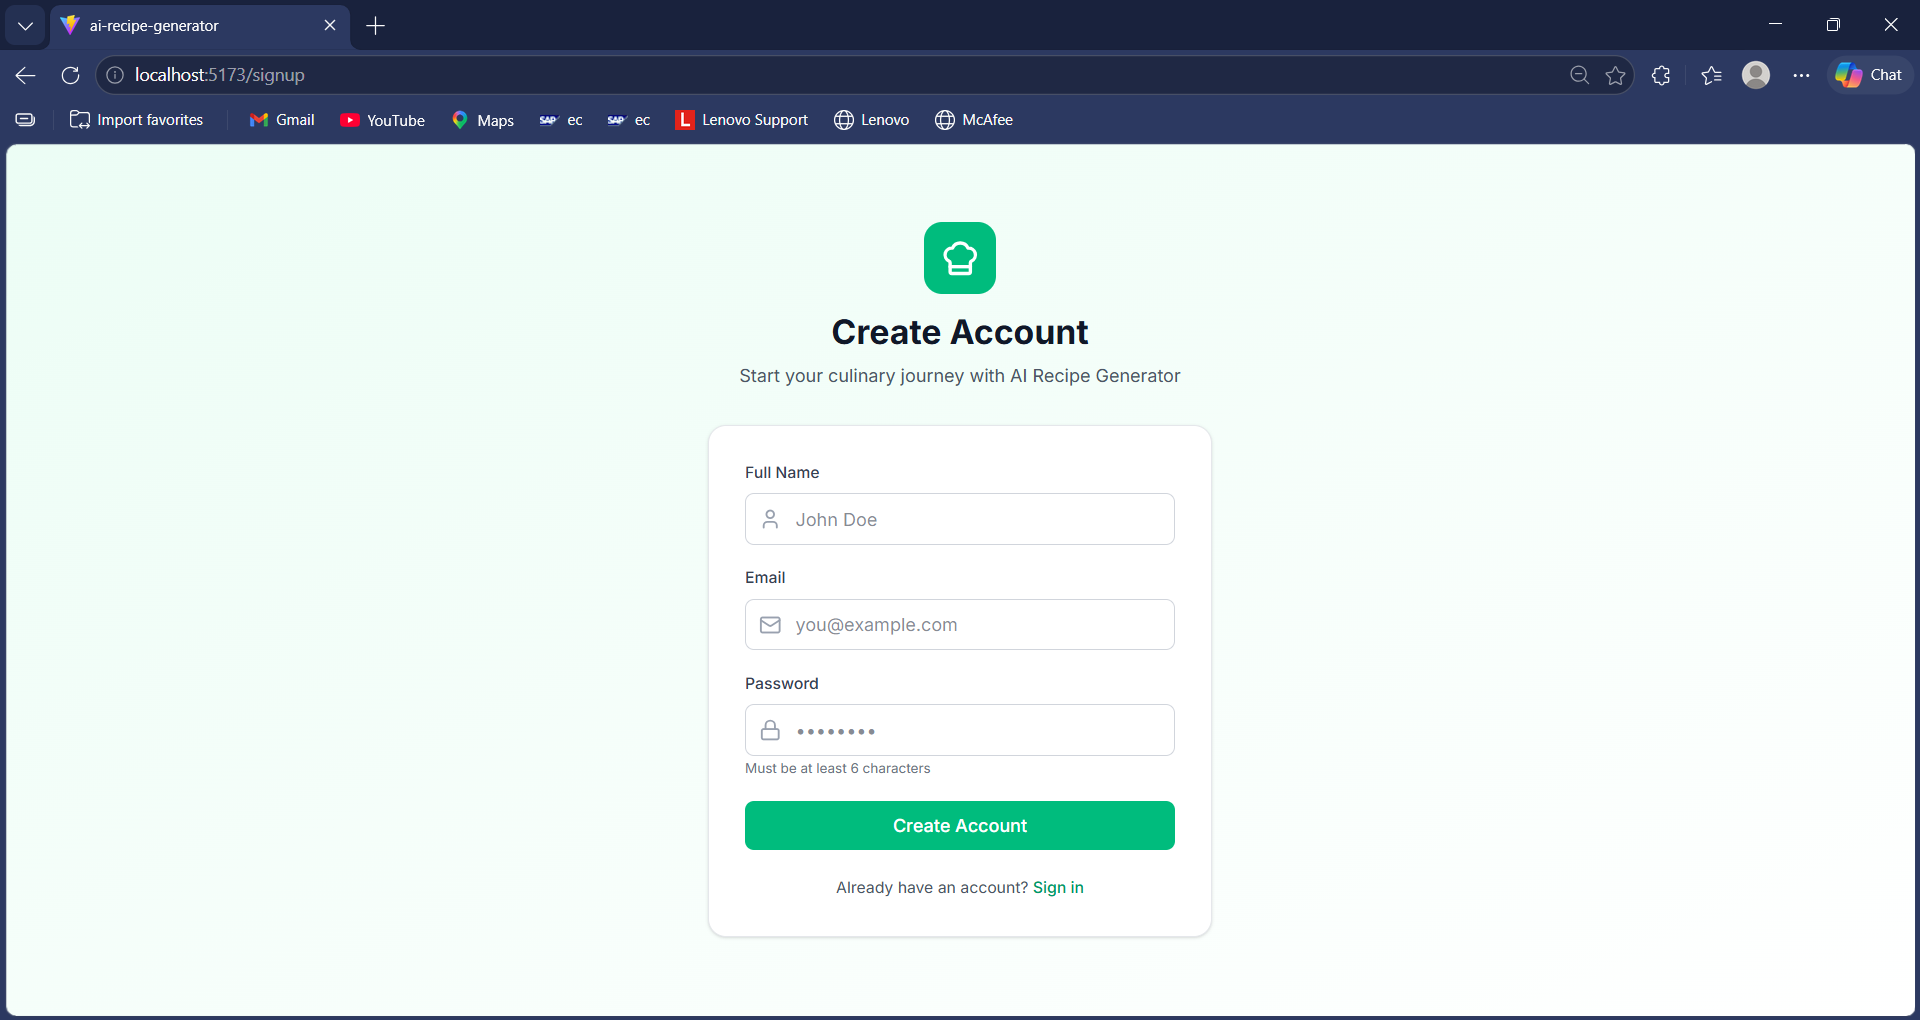
\includegraphics[width=0.78\textwidth,height=0.36\textheight,keepaspectratio]{Screenshot 2026-05-07 223414.png}
    \caption{Account Registration Interface}
    \label{fig:registration_screen}
\end{figure}

\FloatBarrier
\subsection{Dashboard and Recipe Generation}
\begin{figure}[htbp]
    \centering
    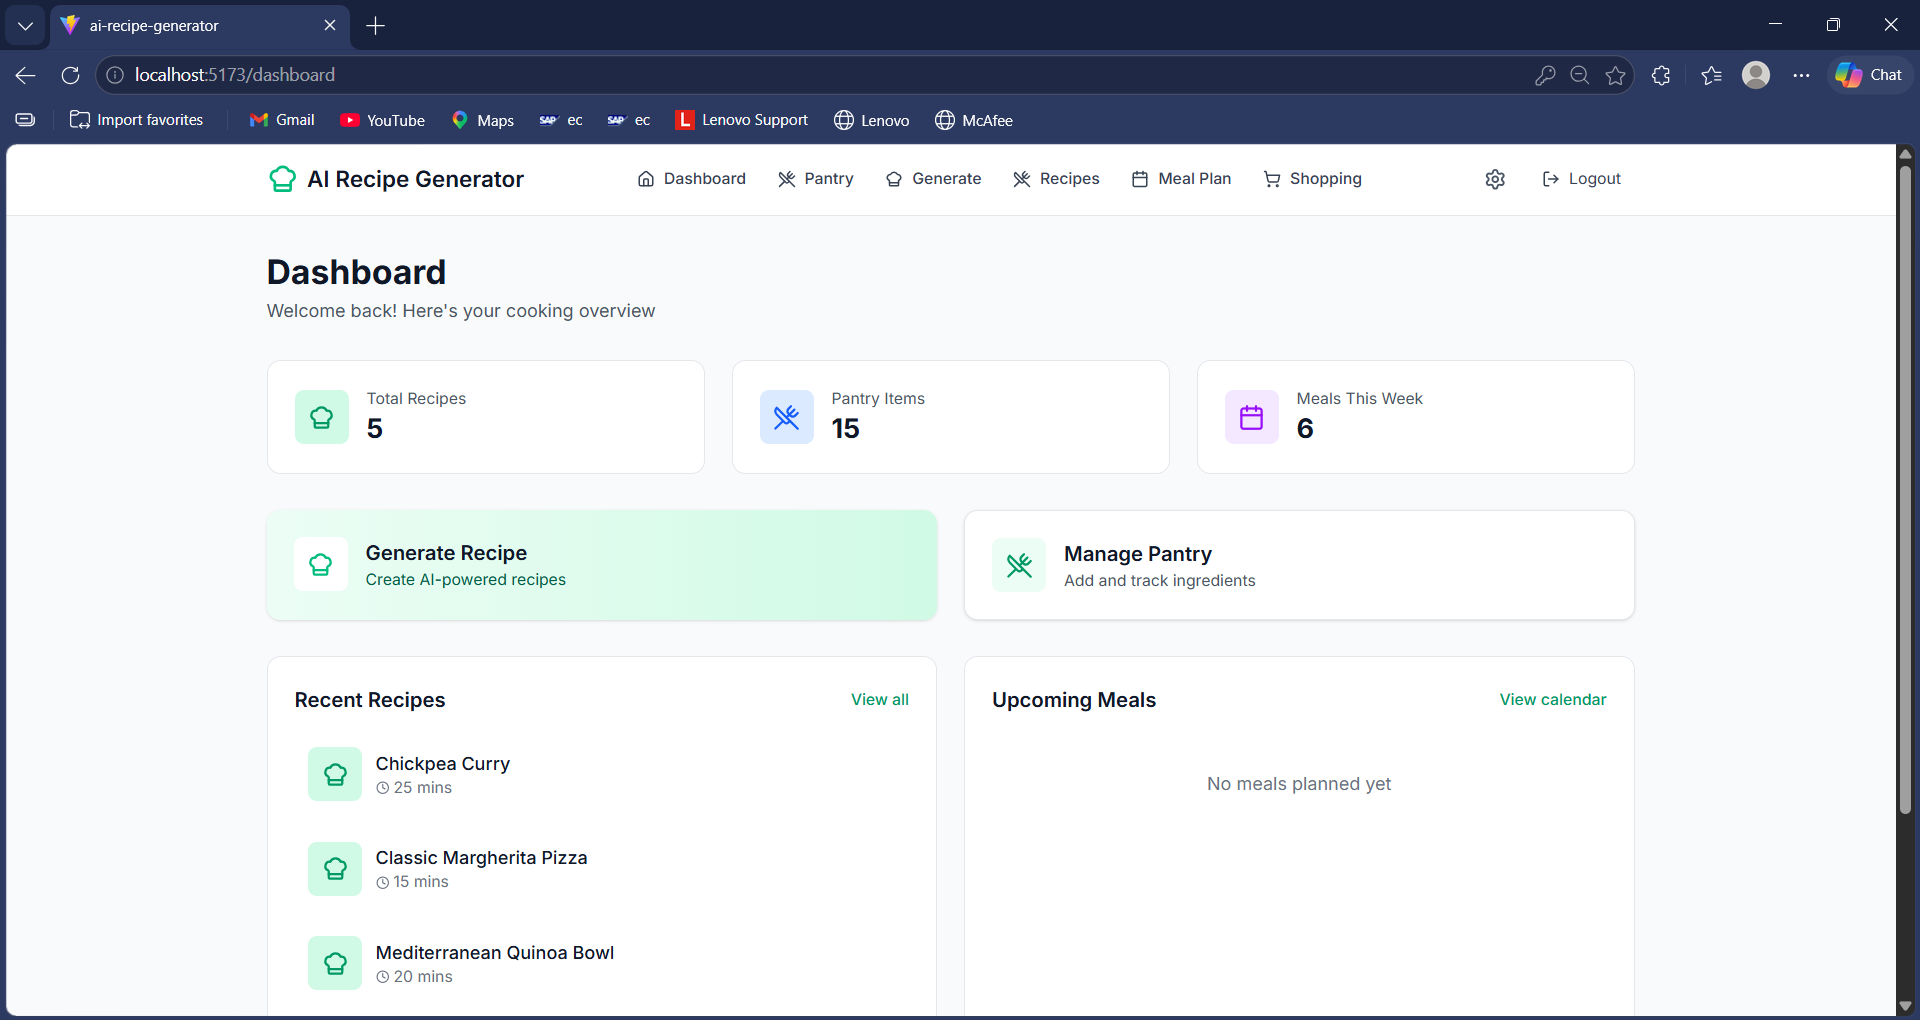
\includegraphics[width=0.78\textwidth,height=0.36\textheight,keepaspectratio]{Screenshot 2026-05-07 223526.png}
    \caption{Main User Dashboard}
    \label{fig:dashboard_screen}
\end{figure}

\begin{figure}[htbp]
    \centering
    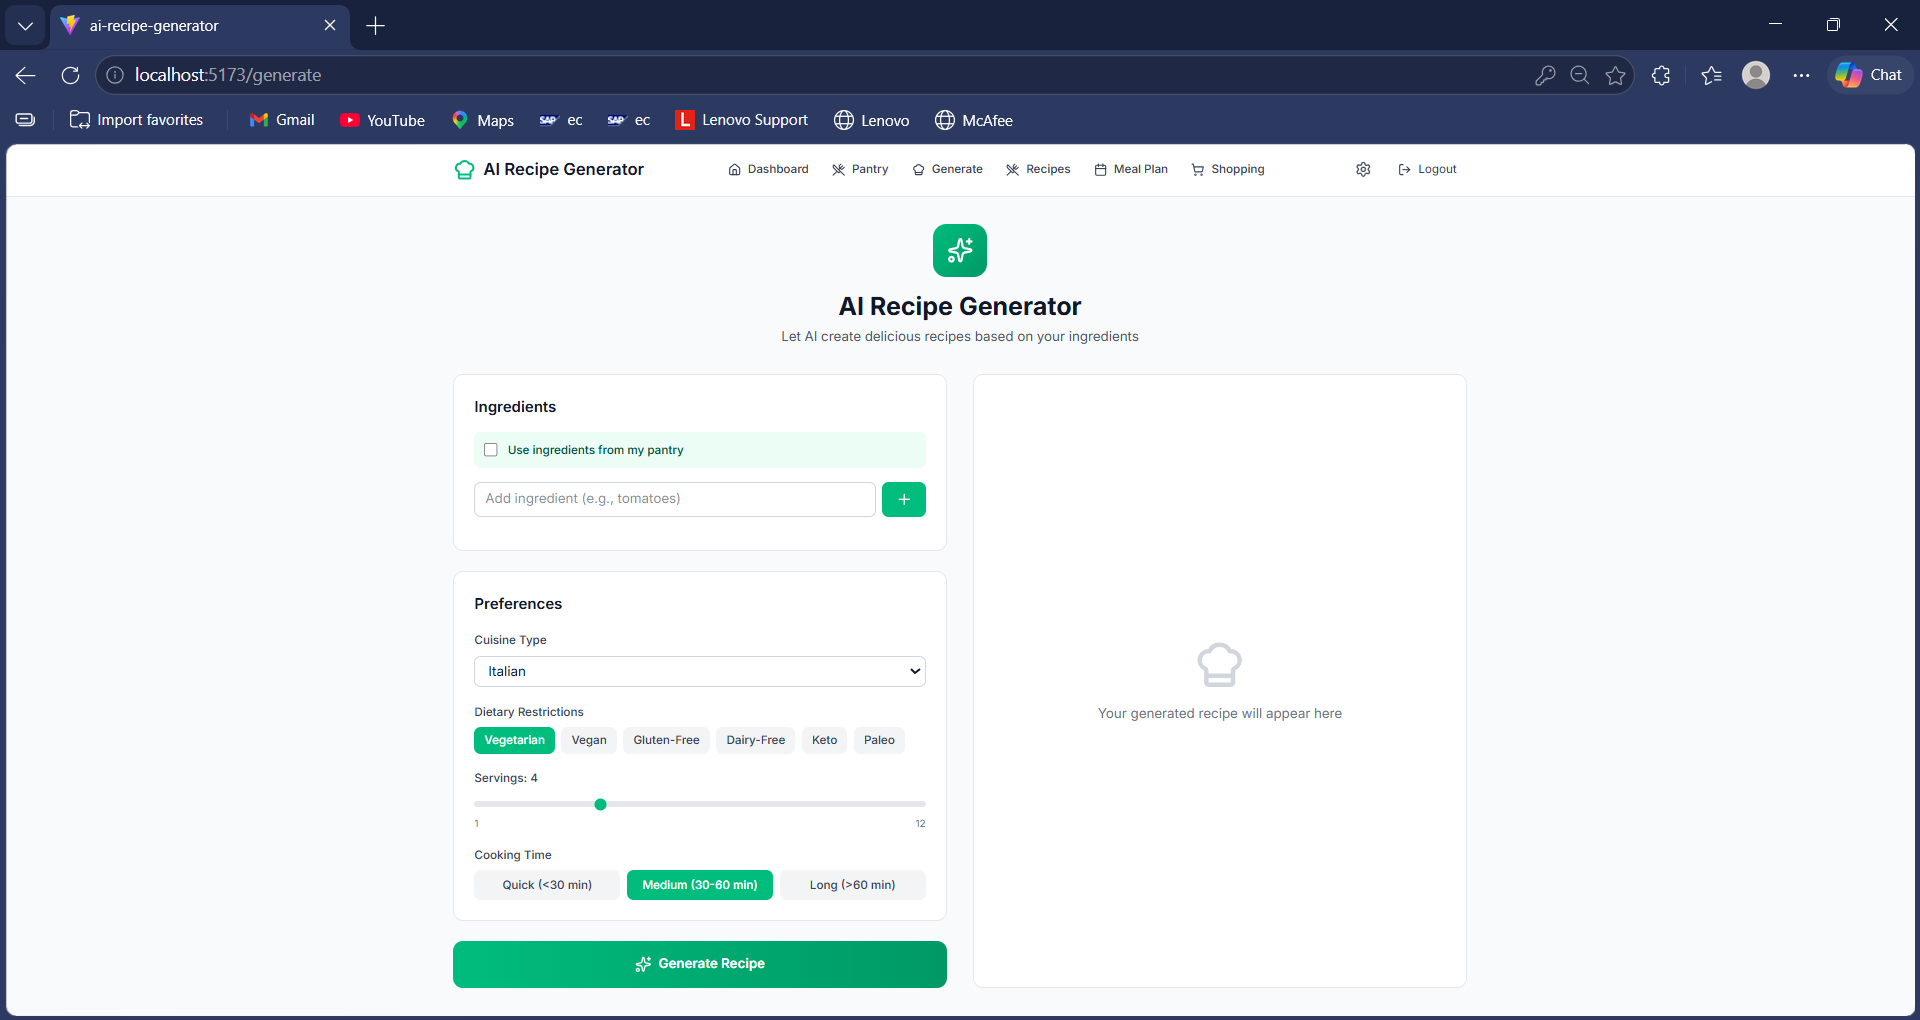
\includegraphics[width=0.78\textwidth,height=0.36\textheight,keepaspectratio]{Screenshot 2026-05-07 223616.png}
    \caption{AI Recipe Generation Interface}
    \label{fig:recipe_generator}
\end{figure}

\FloatBarrier
\subsection{Management and Planning}
\begin{figure}[htbp]
    \centering
    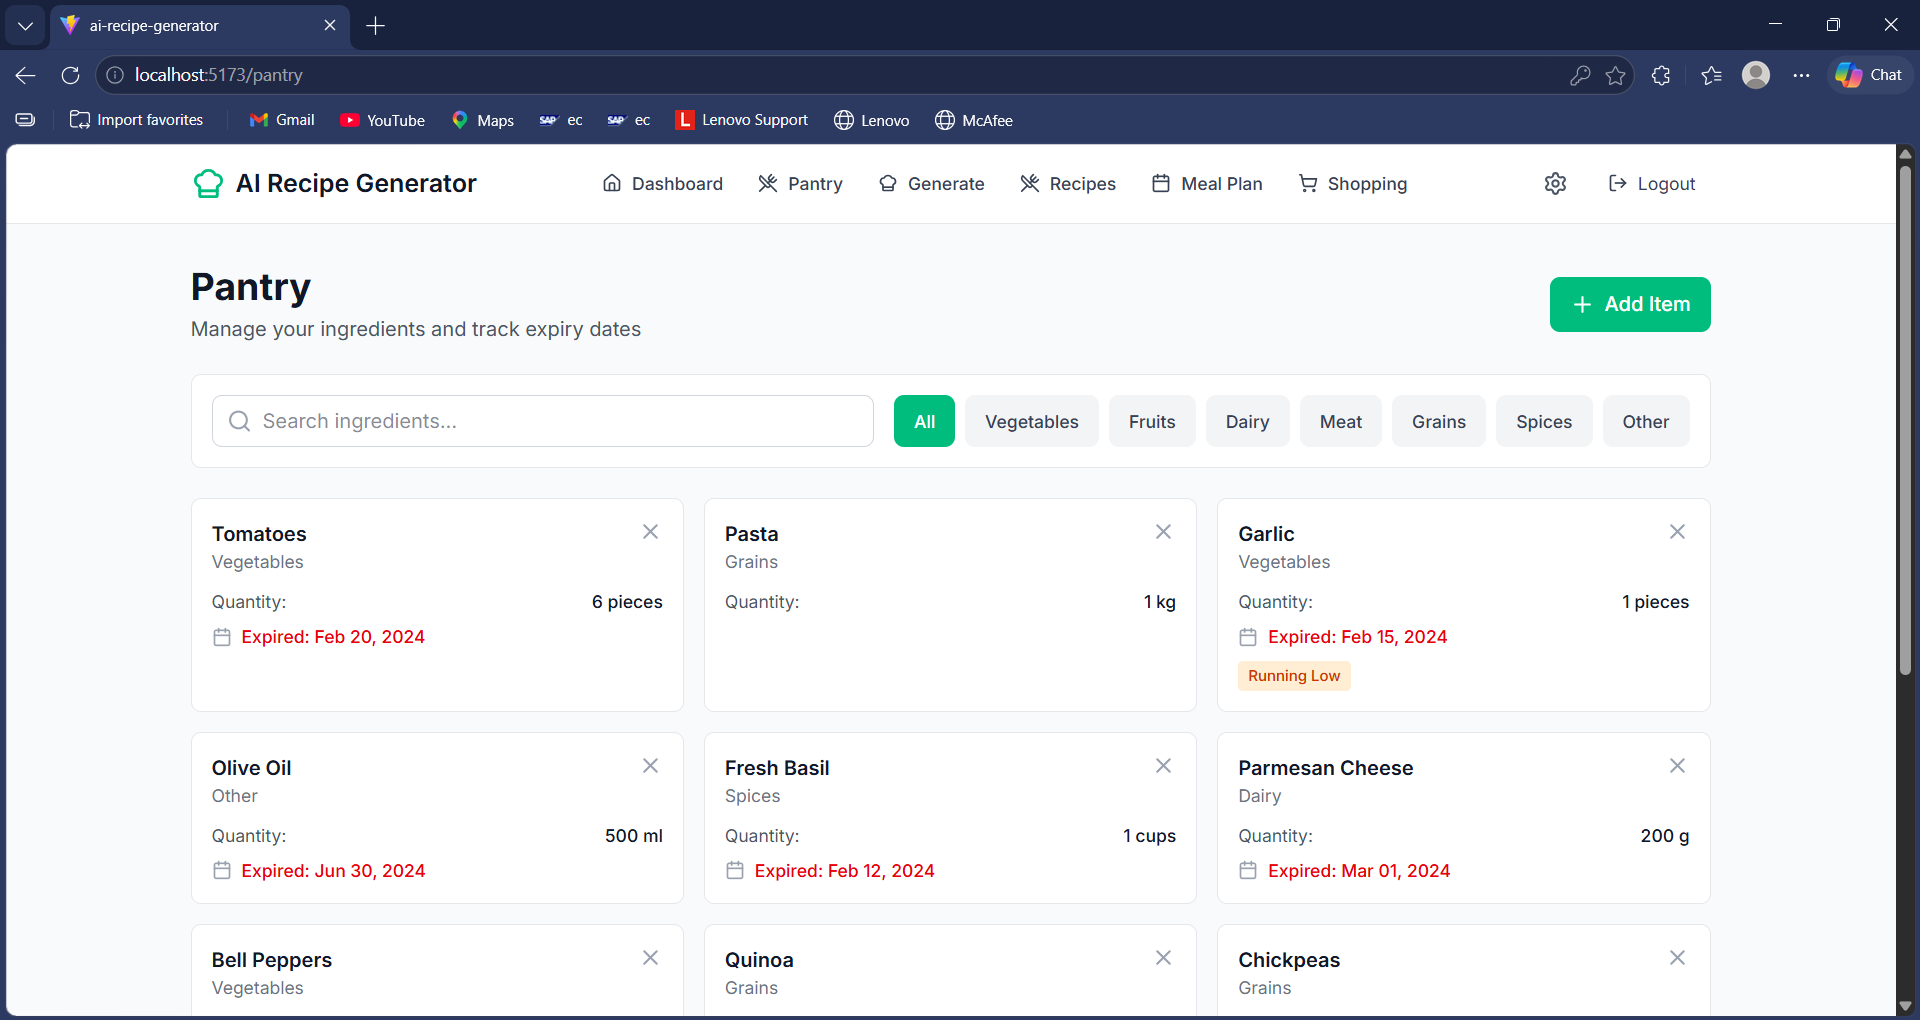
\includegraphics[width=0.78\textwidth,height=0.36\textheight,keepaspectratio]{Screenshot 2026-05-07 223701.png}
    \caption{Pantry Inventory Management}
    \label{fig:pantry_screen}
\end{figure}

\begin{figure}[htbp]
    \centering
    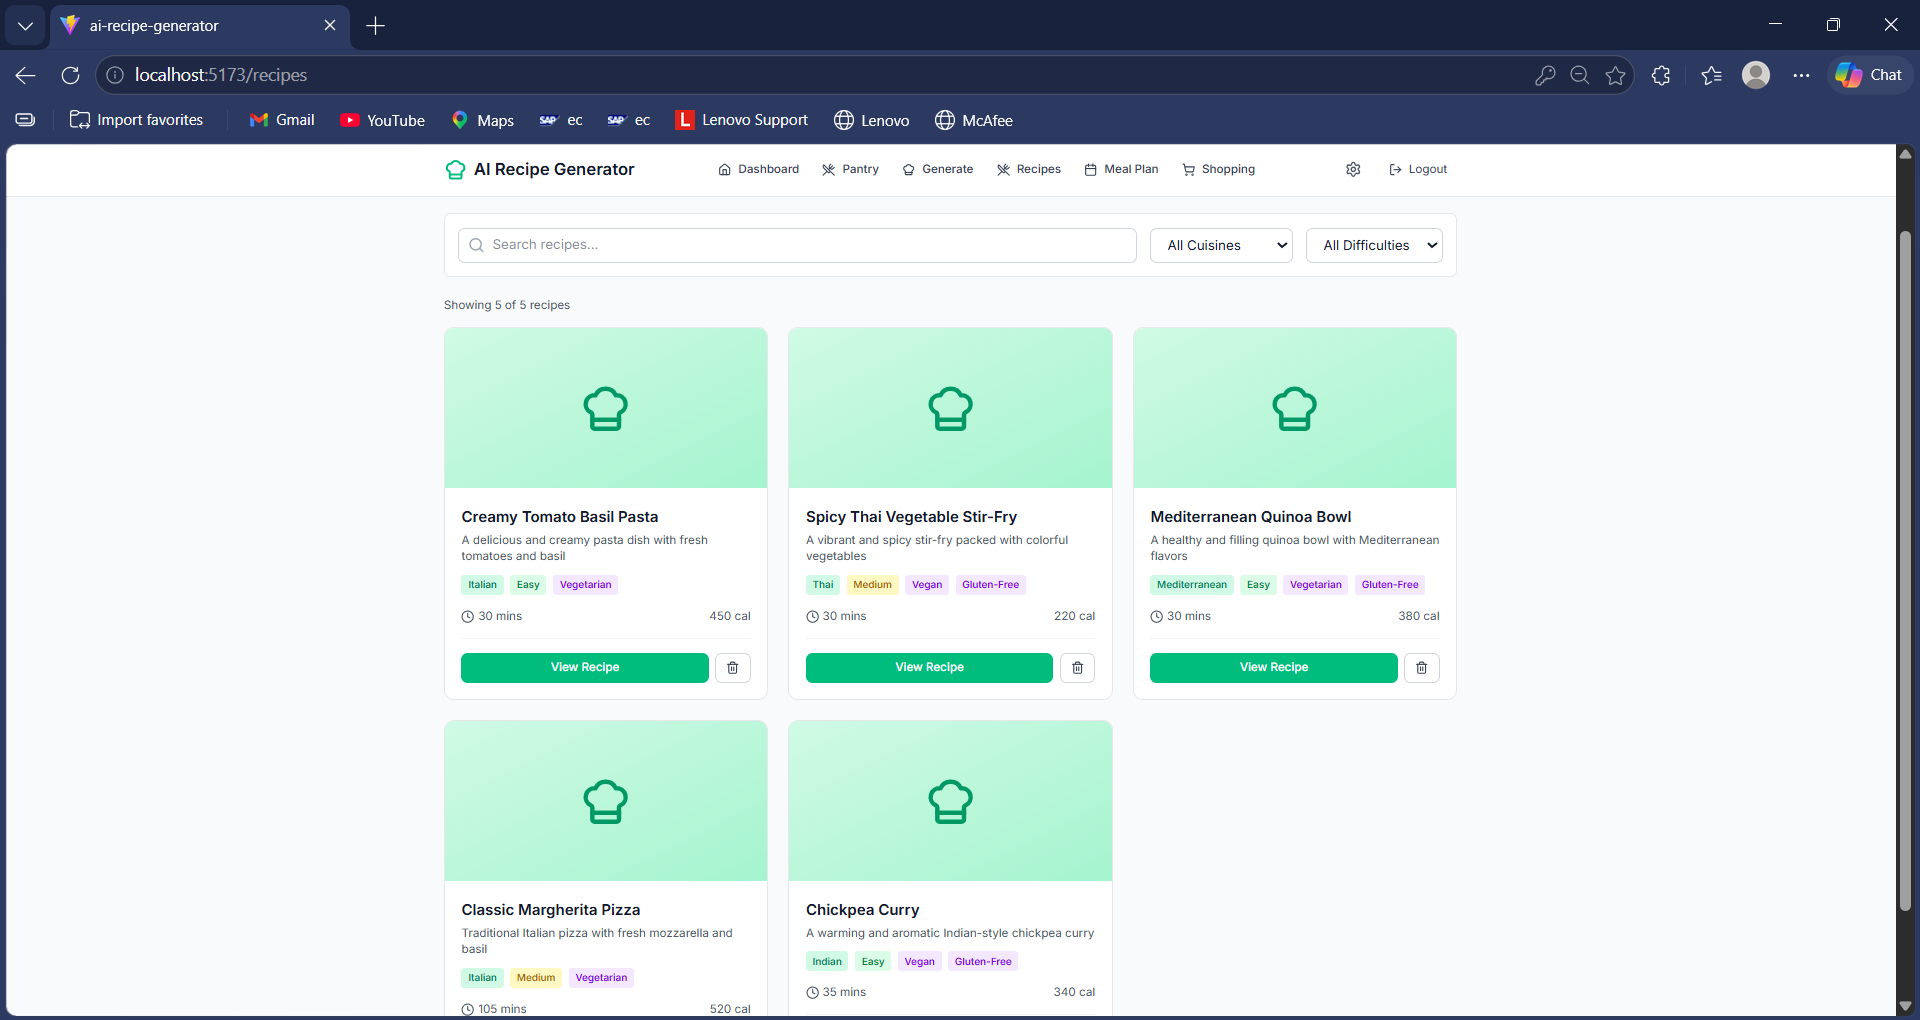
\includegraphics[width=0.78\textwidth,height=0.36\textheight,keepaspectratio]{Screenshot 2026-05-07 223752.png}
    \caption{Collection of Saved Recipes}
    \label{fig:saved_recipes}
\end{figure}

\begin{figure}[htbp]
    \centering
    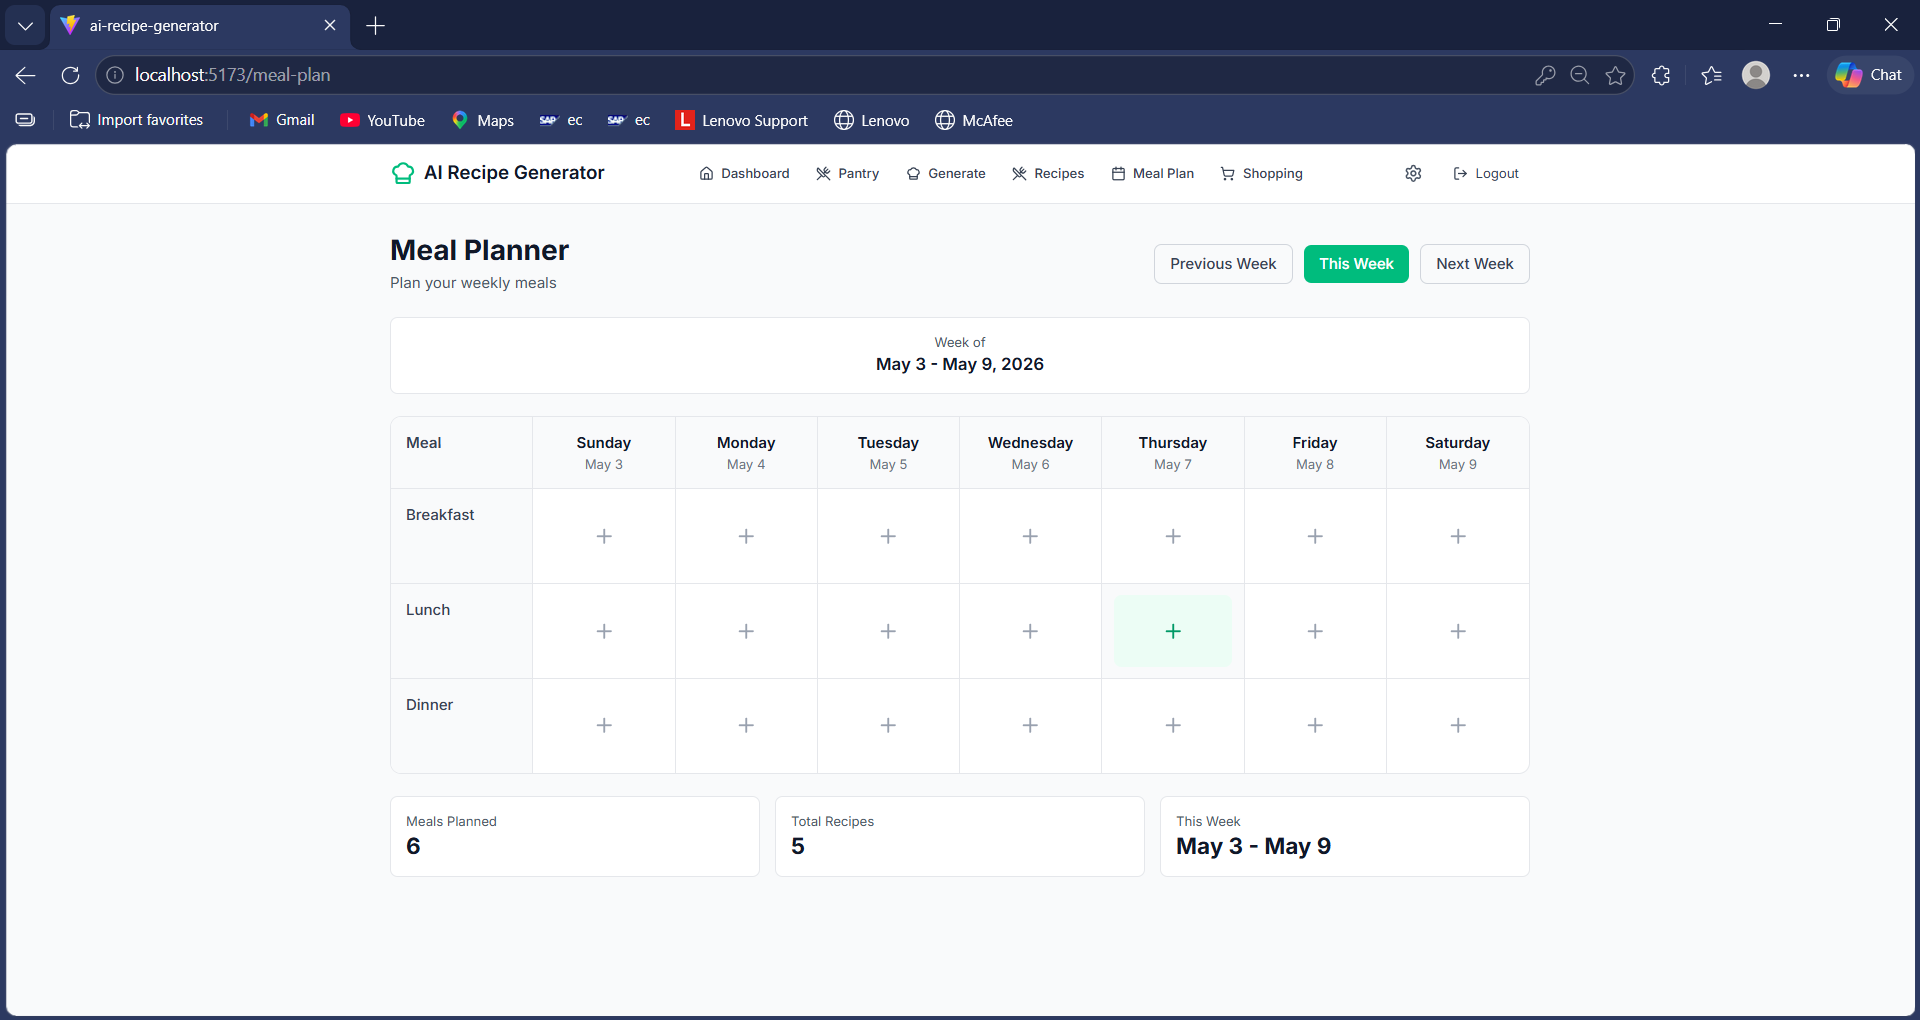
\includegraphics[width=0.78\textwidth,height=0.36\textheight,keepaspectratio]{Screenshot 2026-05-07 223847.png}
    \caption{Weekly Meal Planning Interface}
    \label{fig:meal_planner}
\end{figure}

\begin{figure}[htbp]
    \centering
    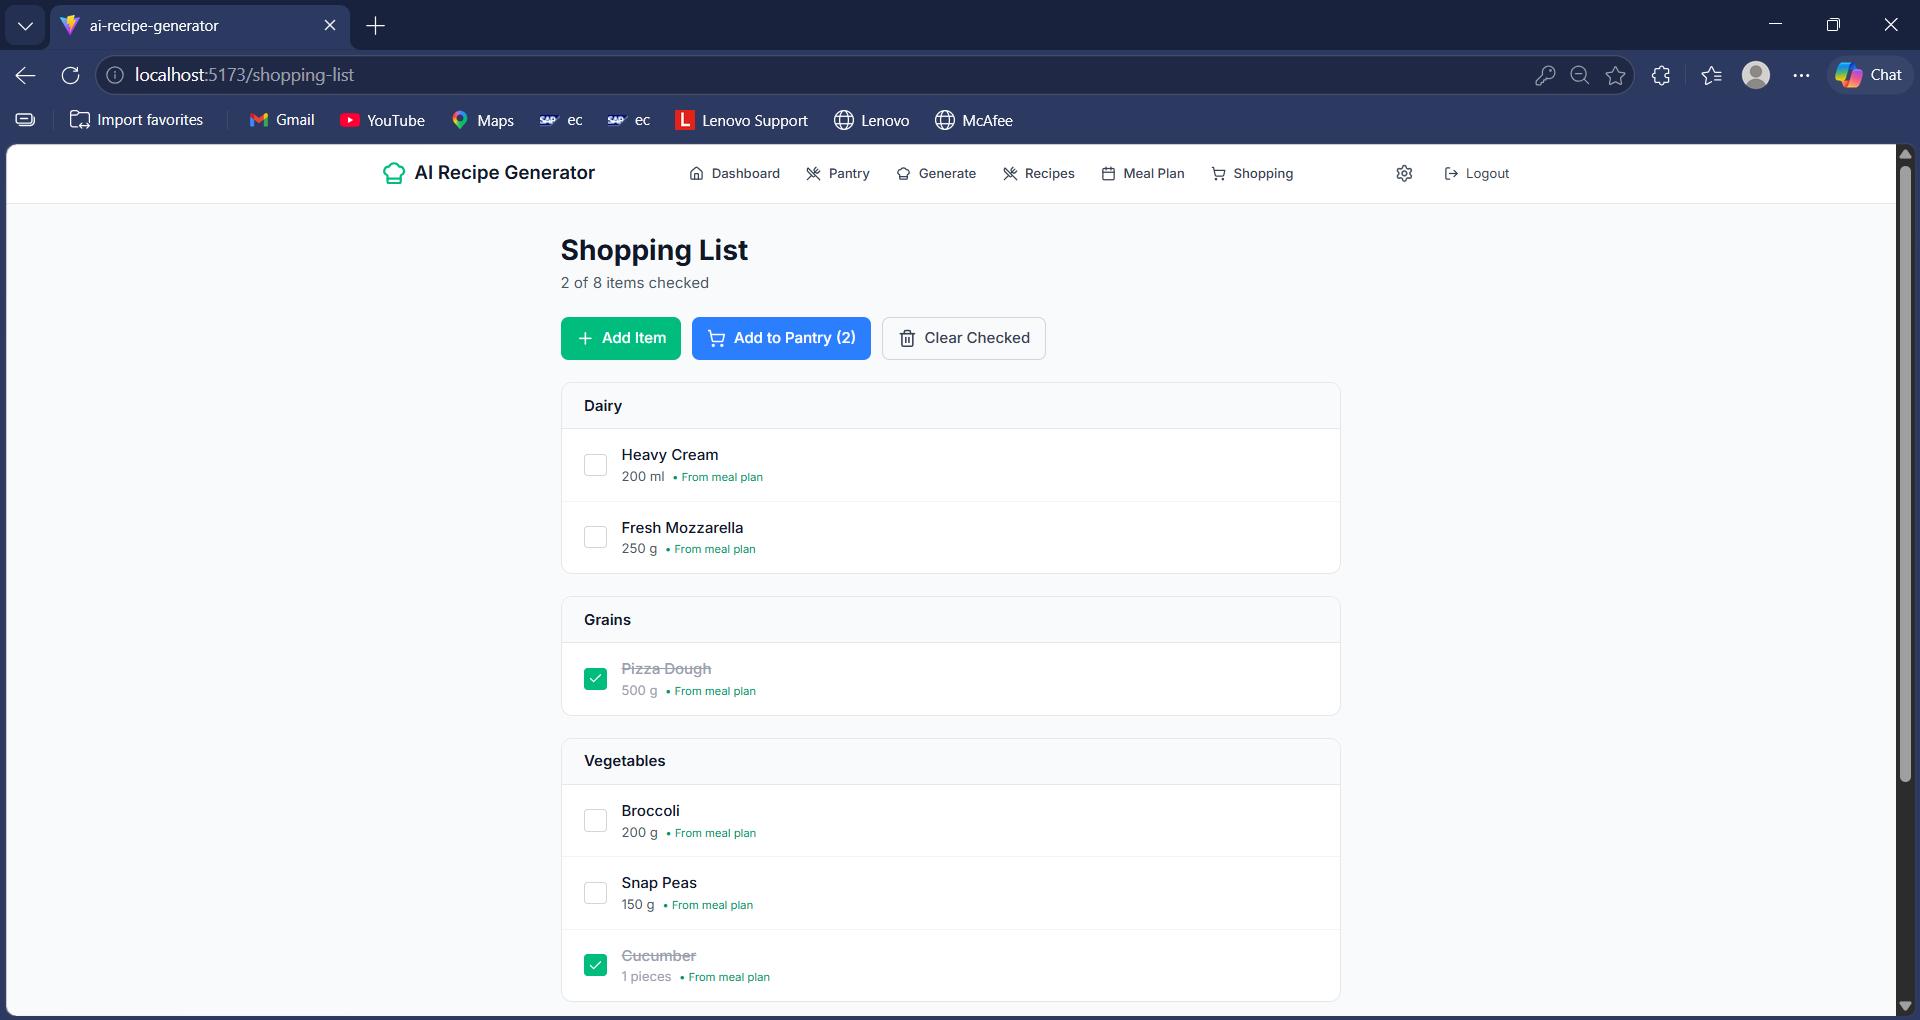
\includegraphics[width=0.78\textwidth,height=0.36\textheight,keepaspectratio]{Screenshot 2026-05-07 224015.png}
    \caption{Automated Shopping List}
    \label{fig:shopping_list}
\end{figure}

\FloatBarrier
\subsection{User Configuration}
\begin{figure}[htbp]
    \centering
    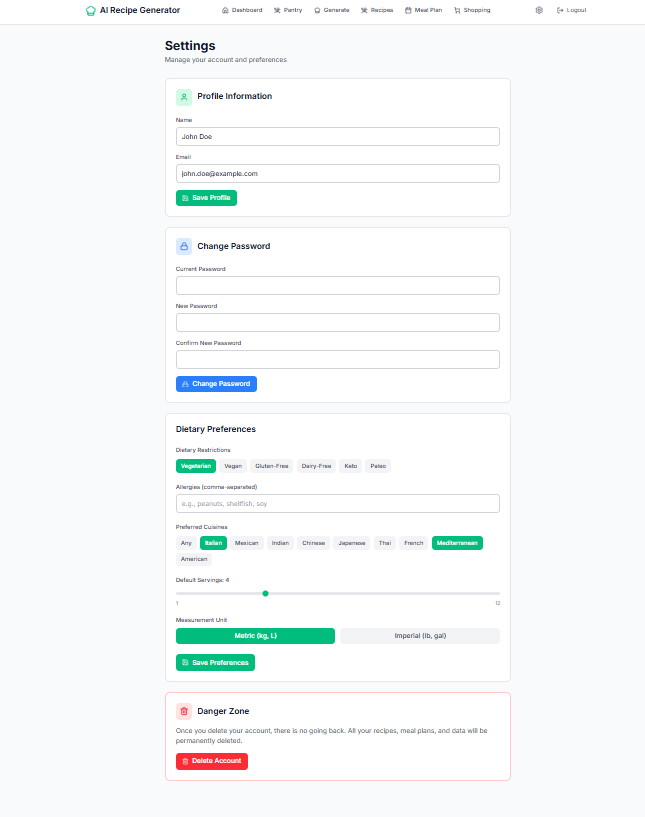
\includegraphics[width=0.78\textwidth,height=0.36\textheight,keepaspectratio]{Screenshot 2026-05-07 224056.png}
    \caption{Application Settings and Profile Management}
    \label{fig:settings_screen}
\end{figure}

\FloatBarrier

\newpage
\section{Conclusion and Future Work}

\subsection{Conclusion}

The AI Recipe Generator project provides a useful web-based solution for users who want to prepare recipes using available ingredients and personal preferences. The system supports user authentication, ingredient entry, recipe generation, pantry management, saved recipes, meal planning, and shopping list preparation. By using React.js for the frontend, Node.js and Express.js for the backend, PostgreSQL for database storage, and Google GenAI/Gemini API for AI-based recipe generation, the project offers a practical and user-friendly cooking assistant.

The system reduces the difficulty of deciding what to cook and helps users make better use of ingredients available at home. It also improves meal organization by allowing users to save recipes, plan meals, and manage shopping items. Overall, the project successfully meets its main objective of generating personalized recipes and supporting daily meal planning activities.

\subsection{Future Work}

In the future, the AI Recipe Generator can be improved with more advanced and intelligent features. Voice-based recipe search can be added so users can interact with the system hands-free while cooking. Image-based ingredient detection can also be implemented, allowing users to upload a photo of available ingredients and generate recipes automatically.

The system can be extended with calorie tracking, nutrition analysis, allergy alerts, recipe sharing, and multilingual support. Mobile application support can also be added for better accessibility. Further improvements may include offline recipe storage, advanced recommendation algorithms, and integration with grocery delivery platforms.
 % adds the Scheduling and Planning page
\newpage

%\input{ref.tex} % adds the References page
\bibliographystyle{IEEEtran}
\begin{thebibliography}{9}

\bibitem{allrecipes}
Allrecipes, ``Recipes, Dinner Ideas and Menus.'' [Online]. Available: \url{https://www.allrecipes.com/}. Accessed: May 11, 2026.

\bibitem{mealime}
Mealime, ``Meal Planning App.'' [Online]. Available: \url{https://www.mealime.com/}. Accessed: May 11, 2026.

\bibitem{react}
Meta Open Source, ``React Documentation.'' [Online]. Available: \url{https://react.dev/}. Accessed: May 11, 2026.

\bibitem{vite}
Vite, ``Vite Documentation.'' [Online]. Available: \url{https://vite.dev/}. Accessed: May 11, 2026.

\bibitem{nodejs}
OpenJS Foundation, ``Node.js Documentation.'' [Online]. Available: \url{https://nodejs.org/en/docs}. Accessed: May 11, 2026.

\bibitem{express}
Express, ``Express.js Documentation.'' [Online]. Available: \url{https://expressjs.com/}. Accessed: May 11, 2026.

\bibitem{postgresql}
PostgreSQL Global Development Group, ``PostgreSQL Documentation.'' [Online]. Available: \url{https://www.postgresql.org/docs/}. Accessed: May 11, 2026.

\bibitem{sequelize}
Sequelize, ``Sequelize Documentation.'' [Online]. Available: \url{https://sequelize.org/docs/v6/}. Accessed: May 11, 2026.

\bibitem{jwt}
Auth0, ``JSON Web Tokens Introduction.'' [Online]. Available: \url{https://jwt.io/introduction}. Accessed: May 11, 2026.

\bibitem{googleai}
Google AI for Developers, ``Gemini API Documentation.'' [Online]. Available: \url{https://ai.google.dev/}. Accessed: May 11, 2026.

\bibitem{tailwind}
Tailwind Labs, ``Tailwind CSS Documentation.'' [Online]. Available: \url{https://tailwindcss.com/docs}. Accessed: May 11, 2026.

\end{thebibliography}


\newpage
\input{Internship.tex}
\addcontentsline{toc}{section}{Internship Report}
\newpage
\section*{Publications}
Details of paper publication: name of the conference/journal, comments of reviewers, certificate, paper
\addcontentsline{toc}{section}{Publication}
\newpage
\input{Plagiarism Report.tex}
\addcontentsline{toc}{section}{Plagiarism Report}
\end{document}
